%template1.tex
%The following LaTeX source file represents the simplest kind of slide presentation; no overlays, no included graphics. Substitute your favorite style for ``pascal''. To create the PDF file template1.pdf, (1) be sure to use the prosper class, then (2) execute the command latex template1.tex, and (3) the command dvipdf template1.dvi.

%%%%%%%%%%%%%%%%%%%%%%%%%%%%%%% template1.tex %%%%%%%%%%%%%%%%%%%%%%%%%%%%%%%%%%%
\documentclass[a4paper,blends,pdf,colorBG,slideColor]{prosper}
% definitions for slides for CSC544
% Lutz Hamel, (c) 2007

\hypersetup{pdfpagemode=FullScreen}

\usepackage{times}
\usepackage{latexsym}
\usepackage{alltt}
\usepackage{booktabs}
\usepackage{amsmath}
\usepackage{amsopn}
\usepackage{amsfonts}
\usepackage{amssymb}
%\usepackage[usenames]{color}

\def\sign{\qopname\relax{no}{sign}}
\def\argmax{\qopname\relax{no}{argmax}}
\def\argmin{\qopname\relax{no}{argmin}}

\newcommand{\grad}{\ensuremath{\nabla}} 
\newcommand{\loss}{\ensuremath{{\cal L}}}
\newcommand{\err}{\mbox{err}}
\newcommand{\mse}{\mbox{mse}}
\newcommand{\acc}{\mbox{acc}}
\newcommand{\Integer}{\ensuremath{\mathbb{N}}}
\newcommand{\size}[1]{{|{#1}|}}
\newcommand{\Rnspace}[1]{\ensuremath{\mathbb{R}^{#1}}}
\newcommand{\Real}{\ensuremath{\mathbb{R}}}
\newcommand{\mytt}[1]{{\small\tt{#1}}}
\newcommand{\textemph}[1]{{\em #1}}
\newcommand{\suchthat}{\mid}
\newcommand{\orbar}{\;|\;}
\newcommand{\bs}[1]{\begin{slide}{#1}\ptsize{8}}
\newcommand{\es}{\end{slide}}
\newcommand{\co}{\,\colon\;}
\newcommand{\pair}[2]{\ensuremath{( {#1}, {#2} )}}
\newcommand{\model}[1]{\hat{#1}}
\newcommand{\ul}[1]{{\bf\em #1}}
\newcommand{\ol}{\overline}
\newcommand{\definition}[1]{{\bf Definition: }{\em #1}}
\newcommand{\example}[1]{{\bf Example: }{#1}}
\newcommand{\abs}[1]{|{#1}|}
\newcommand{\mytab}{\makebox[.1in]{}}

\newcommand{\fdef}[1]{
\begin{center}
\fbox{
\begin{minipage}{3.5in}
{\bf Definition:}
{#1}
\end{minipage}
}
\end{center}
}

\newcommand{\fframe}[1]{
\begin{center}
\fbox{
\begin{minipage}{3.5in}
{#1}
\end{minipage}
}
\end{center}
}

\newcommand{\nframe}[1]{
\begin{center}
\begin{minipage}{3.5in}
{#1}
\end{minipage}
\end{center}
}

\newenvironment{Rcode}
	{
		\scriptsize
		\begin{quote}
		\begin{alltt}
	}
	{
		\end{alltt}
		\end{quote}
	}




\begin{document}

\bs{ANN in R}
Let's take a look at ANN's in R.  The 'neuralnet' package works nicely and has
a nice visual representation of the ANN's built.

\vspace{.2in}

We will start building a neural network for classifying Iris flowers.
\es

\bs{ANN in R}
Train our ANN
\scriptsize
\begin{verbatim}
# load our data set
data(iris)

# make sure the ANN library is available
library(neuralnet)

# convert the labels into numeric labels and put them into a data frame
Species.numeric <- as.numeric(iris$Species)
iris.df <- data.frame(iris,Species.numeric)

# train a neural network with two hidden nodes
net <- neuralnet(
    Species.numeric ~ Sepal.Width+Sepal.Length+Petal.Width+Petal.Length,
    iris.df,
    threshold=0.01,
    stepmax="10000",
    lifesign="none",
    hidden=2)
\end{verbatim}
\es


\bs{ANN in R}
The data set:
\scriptsize
\begin{verbatim}
> iris.df[1:5,]
  Sepal.Length Sepal.Width Petal.Length Petal.Width Species Species.numeric
1          5.1         3.5          1.4         0.2  setosa               1
2          4.9         3.0          1.4         0.2  setosa               1
3          4.7         3.2          1.3         0.2  setosa               1
4          4.6         3.1          1.5         0.2  setosa               1
5          5.0         3.6          1.4         0.2  setosa               1
> levels(iris.df$Species)
[1] ``setosa''     ``versicolor'' ``virginica'' 
\end{verbatim}
\es

\bs{ANN in R}
Evaluate our ANN
{
\scriptsize
\begin{verbatim}
# display the ANN
plot(net)

# the training predictions from the ANN are numeric values, 
# turn them into labels by rounding
predicted.labels <- round(net$net.result[[1]])

# plot the confusion matrix
print(table(iris.df$Species.numeric,predicted.labels))
\end{verbatim}
}

\vspace{.2in}
The Confusion Matrix
{
\scriptsize
\begin{verbatim}
   predicted.labels
     1  2  3
  1 50  0  0
  2  0 49  1
  3  0  1 49
\end{verbatim}
}

\es

\bs{ANN in R}
\begin{center}
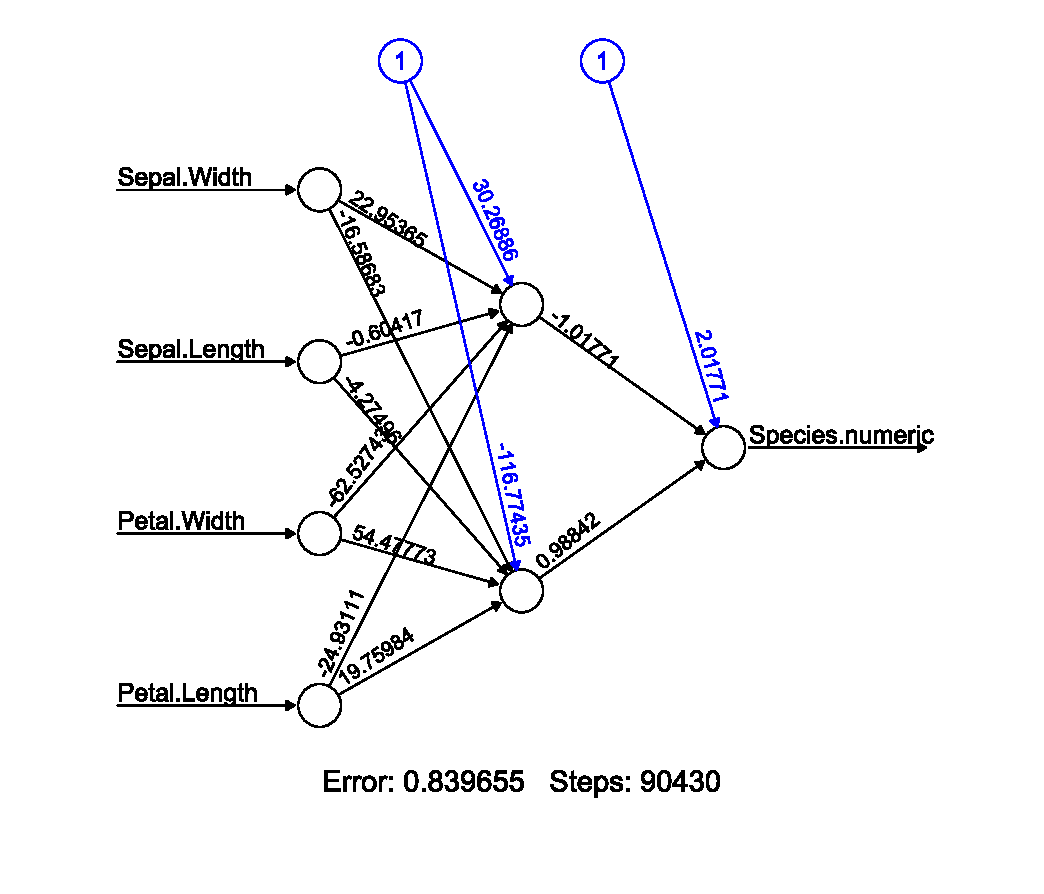
\includegraphics[height=60mm]{images/ann-plot.eps}
\end{center}
\es

\bs{ANN in R}

Demo...

\es

\end{document}
%%%%%%%%%%%%%%%%%%%%%%%%%%% end of template1.tex %%%%%%%%%%%%%%%%%%%%%%%%%%%%%%%%

